\section{Text and Code}

This section starts with a look at the text as a learning material that humans produce and consume, continues with a production of a source code from the viewpoint of a learner, and ends with a short subsection on how the code is processed by a machine.

\subsection{Producing Learning Material}

For the purposes of this thesis, we can simplify the choice of a way to produce learning material by considering two approaches:

\begin{enumerate}
    \item \gls{wysiwyg} editors like Microsoft Word and PowerPoint or Adobe Dreamweaver and Captivate.
    \item Plain text formats like \LaTeX, HTML, or Markdown and the tools that are necessary to make them usable.
\end{enumerate}

The first group of tools is commonly mentioned when presenting authoring tools for learning content \parencite{khademi_review_nodate}.
While most of these tools are said to be easy to use and often concentrate on creating courses, the majority of them are also paid, and there are concerns about interoperability \parencites{khademi_review_nodate}{shieber_why_2014}.
One particular concern mentioned by \textcite{shieber_why_2014} is the lack of output consistency when different users use the large range of functionality of these tools differently.

Compared to the problems with the input of \gls{wysiwyg} editors mentioned above, plain text input is by nature backwards compatible and interoperable as it is largely a UTF-8 encoded text \parencite{shieber_why_2014}.
However, the complexity of plain text formats can differ considerably.
LaTeX, which is used extensively within the scientific community, is commonly understood to be more powerful and complex, carries larger overhead on the input, and can potentially take longer to write \parencites{baramidze_latex_2013}{knauff_efficiency_2014}{shieber_why_2014}.
One of the most common specifications of Markdown, Commonmark, features a two-page long self-explanatory reference guide\footnote{Available at \url{https://commonmark.org/help/}.} while LaTeX distributes a 31-page long user guide\footnote{Available at \url{https://www.latex-project.org/help/documentation/usrguide.pdf}.}.
Moreover, Markdown is said to have a lower overhead than both LaTeX and \gls{html} \parencite{shieber_why_2014} while still permitting extensibility with LaTeX-like features \parencite{shieber_why_2014} and allowing for potentially better accessibility \parencite{voegler_markdown_2014}.
The output format LaTeX and Markdown focus on seems clear from the respective websites.
While the LaTeX project website\footnote{Available at \url{https://www.latex-project.org}.} commonly mentions PDF as the output format, Commonmark specification\footnote{Available at \url{https://spec.commonmark.org/0.30/}.} directly mentions \gls{html} as the expected output.
\gls{html} output is possible with LaTeX as well, but the efficiency of the most commonly used tool\footnote{LaTeX2HTML available at \url{https://www.latex2html.org/}.} is limited as the produced \gls{html} is said to be often substandard \parencite{voegler_markdown_2014}.

\subsection{Writing Code}

According to a survey conducted by \textcite{StackOverflow_2023}, more complex \glspl{ide} like Visual Studio Code, Visual Studio, or IntelliJ IDEA are used by more developers than simpler text editors like Notepad++ or Vim.
The most popular \gls{ide} used by more than 70\% of professionals and learners is Visual Studio Code \parencite{StackOverflow_2023}.

Research focusing on the ease of use of sophisticated \glspl{ide}, especially among learners, is inconclusive.
While a survey from \textcite{owoseni_2016} suggests learners find sophisticated \glspl{ide} difficult to use when learning programming, \textcite{vihavainen_how_2014} use session traces to back the opinion there is no evidence learning to use an \gls{ide} is hard.

As far as a web-based \gls{ide} goes, \textcite{valez_student_2020} explored the idea of using a pre-configured custom \gls{ide} that is a low-threshold alternative to common \glspl{ide}.
While most participants found the web \gls{ide} useful and found the fact that it was web-based and did not require installation useful, it was also found to often lack the functionality learners were looking for and was used mostly by more junior students \parencite{valez_student_2020}.

\subsection{Parsing Code}

This subsection starts with a mention a subset of basic graph terminology relevant for this thesis and some basic algorithms and graph properties.
After a brief introduction to graph theory, it is possible to talk about tokenizers and parsers from a practical point of view of a software developer.

\subsubsection{Graph Theory}

A graph is a data structure that consists of a non-empty finite set of \emph{vertices} and a possibly empty finite set of \emph{edges} \parencite{wilson_graph_2009}.
Each edge connects exactly two vertices, and if the edges have a direction, we call the graph a \emph{directed} graph \parencite{wilson_graph_2009}.

There are many different ways how to traverse a graph.
One such way is to use the \gls{bfs} algorithm.
\gls{bfs} follows the following logic \parencite{wilson_graph_2009}:

\begin{enumerate}
    \item Take a vertex \emph{v}.
    \item Visit all vertices that have an incoming edge from \emph{v}.
    \item Repeat step 1. with the least recently visited \emph{v} from which we did not yet visit other vertices.
\end{enumerate}

If we can find a path through the graph that starts and ends with the same vertex, it is said it contains a \emph{cycle} \parencite{wilson_graph_2009}.
In case some vertex has no associated edges, it is an \emph{isolated vertex}, and if it is not possible to visit all vertices via edges from each vertex, the graph is called \emph{disconnected} \parencite{wilson_graph_2009}.
Figure~\ref{fig:text-graph-basics} shows an example graph that is disconnected as there is no edge connecting $J$ with the rest of the graph.
Additionally, it is cyclic, as vertex $DF$ creates a cycle that could be removed by removing one of the edges $DE$, $EF$, or $DF$.

\begin{figure}[H]
    \centering
    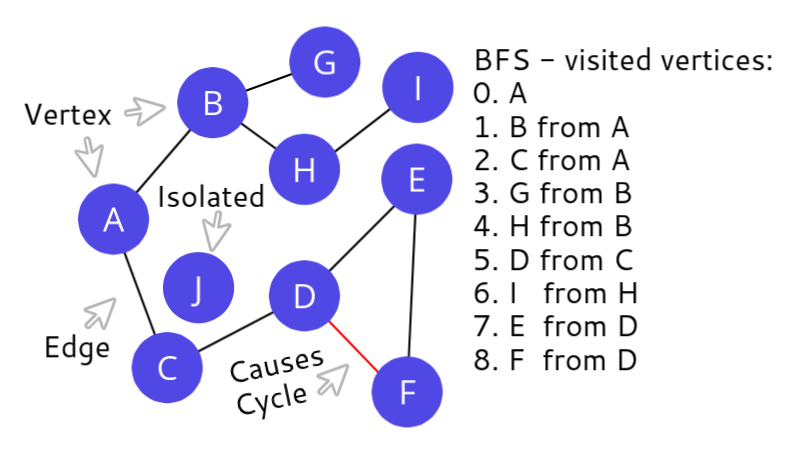
\includegraphics[height=8cm, keepaspectratio]{Graph_Basics}
    \caption{Example disconnected graph showing different concepts.}
    \label{fig:text-graph-basics}
\end{figure}

A graph is considered a \emph{tree} if it has exactly one path between any of the vertices, does not contain cycles, and is not disconnected \parencite{wilson_graph_2009}.
A tree is called \emph{rooted} if exactly one vertex is chosen as the root and all edges are "directed away from the root" \parencite{Baek_trees_2015}.
Figure~\ref{fig:text-tree-basics} shows an example of such a tree.
Vertices that have at least one outgoing edge are called \emph{internal vertices}, while vertices that have no outgoing edge are called.
\emph{Children} of an internal vertex are all vertices that have an incoming edge from that internal vertex \parencite{Baek_trees_2015}.

\begin{figure}[H]
    \centering
    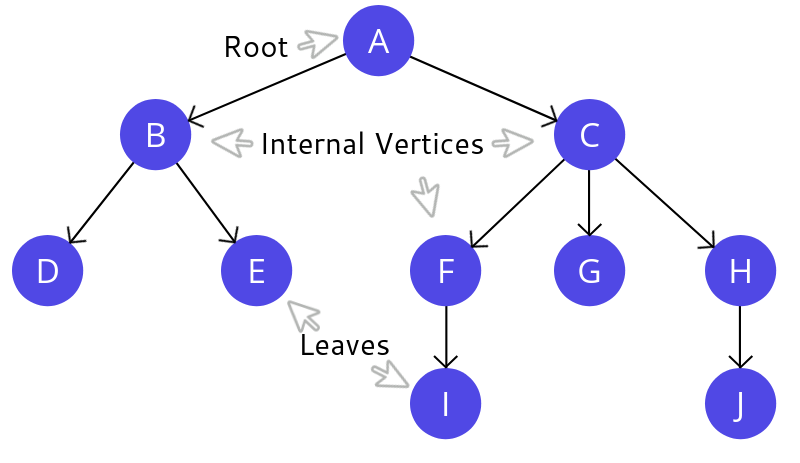
\includegraphics[height=8cm, keepaspectratio]{Tree_Basics}
    \caption{Example directed rooted tree.}
    \label{fig:text-tree-basics}
\end{figure}

\subsubsection{Tokenizers and Parsers}

\todo[inline]{Is referencing fine here? How to cite sources if I've only loosely used \parencites{tomassetti_parsing_2017}{Kjolstad_parsing_2023} as most of the literature is too theoretical and "unwieldy"?}

Parsing is a process of turning a text in a given \emph{language}, like code, into some meaningful object, for example, a program that can be executed \parencites{tomassetti_parsing_2017}{Kjolstad_parsing_2023}.
A naive approach to parsing is to go through the program character by character using a loop.
However, the logic of our language, called \emph{grammar}, would have to be captured within the procedural code, which would make it rather verbose, inflexible, and relatively hard to understand.
Instead, the grammar of the language is commonly defined separately and serves as an input for a \emph{parser generator}, which creates the parser.
The parser can operate on individual characters, in which case it is said to be \emph{scannerless} as it lacks a \emph{scanner} that would pre-process the text.
The scanner groups individual characters into more meaningful tokens and, for the purposes of this thesis, is also referred to as \emph{lexer} or \emph{tokenizer}.

Therefore, we can say processing of the text on the input goes through three distinct consecutive phases:

\begin{enumerate}
    \item \textbf{Lexing}: A string of characters on the input is broken down using a lexer into a string of tokens.
    \item \textbf{Parsing}: A string of tokens on the input is turned into a \gls{cst} using a parser - if the input is valid.
    \item \textbf{Processing}: A valid \gls{cst}, which is mostly just a set of tokens represented using a tree, is simplified into an \gls{ast}, which is a convenient logical representation of the described object.
\end{enumerate}

From a practical point of view, lexing is typically done using regular expressions as it is the simplest sufficient way to define a regular language used for tokens.
Moreover, the processing of parsed tokens can usually be done during the parsing, rather than after, skipping the extra tree traversal.
Therefore, parser generators can take: 1. one or more regular expressions defining tokens, 2. grammar, and 3. processing rules on the input and produce encapsulated parser abstraction capable of performing all three mentioned steps.
As such, the produced parser takes text on the input and provides the \gls{ast} on the output.

Since the job of a lexer and parser generator is rather generic, these are abstracted away by a library or a set of libraries.
The specification of grammar is left to a human, and the supported features differ between different types of parser generators.
A commonly used feature is recursion within the grammar rule.
A special case is a left and right recursion when the rule refers to itself on the leftmost or rightmost part of the rule.

Whether a given grammar can be written concisely and the performance of the generated parser is sufficient are typical deciding factors when choosing a parser generator.
Conciseness allowed by using features like left and right recursion may require a higher complexity that can mean a worse performance depending on the use case.
Simpler and faster parsers called \emph{LL} parse from left to right and produce a tree from the largest logical blocks to the smallest logical blocks called \emph{terminals}.
More flexible but potentially slower are parsers using the \emph{Earley} algorithm.
Earley algorithm uses top-down dynamic programming and enables support of both left and right recursion, and allows for ambiguous grammar.
While the average performance of an Ealery parse is $\theta(n^3)$, where $n$ is the number of tokens on the input, there are multiple ways to achieve better performance (and complexity class): by using left recursion, by using unambiguous grammar, or by using an implementation that features optimizations from \textcite{leo_general_1991} if using right recursion in an LL grammar.
